\newpage

\titleformat % design des titres des chapitres
{\chapter}
[display]
{\centering\normalfont\Large\scshape\bfseries}
{\rule[3pt]{0.15\linewidth}{3pt}\quad\chaptertitlename~\thechapter\quad \rule[3pt] {0.15\linewidth}{3pt}}
{0\baselineskip}%espace vertical entre chapitre et nom du chapitre
{\rule{\linewidth}{0.5pt}\break\Huge}
[\vspace{-0.5\baselineskip}\rule{\linewidth}{0.5pt}\vspace{0\baselineskip}]

\let\clearpage\relax% Stop LaTeX from going to a new page; and
\vspace*{5.5cm}%

\chapter{Etude generale du projet}
Le présent chapitre a pour but de définir les clés du travail
d’identification et planification du projet.

\newpage

\section{Périmètre du projet}
\subsection{Problématique générale}

Actuellement, il n’existe aucune solution pour le suivi d’une pipe commerciale. La méthodologie utilisée pour l’instant est basée sur plusieurs fichiers Excel qui sont partagés entre plusieurs entités. Il est pertinent de libérer ce style classique adopté par les commerciaux et les responsables des ressources humaines qui est basé sur le calcul manuelle des couts ainsi que l'utilisation excessive d'Excel pour classifier tous les acteurs matériaux ou humanitaires qui participent dans la construction d’un « Deal ». 
\\

Donc notre problématique majeure est de définir d’une manière claire et précise les besoins et les attentes d’un système d’information permettant d’automatiser les remontées de l’équipe vers différentes entités, ainsi que la saisie des Deals, choix des Squads, l’affectation des ressources et aussi la gestion de la relation client. D’une autre part garder la trace de tous les échanges afin de pouvoir établir des statistiques ainsi que des tableau de bord pour prendre la décision du gain du deal.

\subsection{But du projet}

Le but de ce projet est de réaliser une solution Power Platform pour la facilitation et la gestion du système d’information. Un outil qui va permettre de digitaliser le processus de gestion de Pipe commercial et de se libérer de l’utilisation exagéré des fichiers Excel pour passer vers l’utilisation de base de données plus robuste et efficace. L’application a pour vision de :  
\\

\begin{itemize}
  \item Un contrôle efficace des coûts ce qui explique l'utilisation d'une plate-forme robuste capable de rassembler des données à partir de différentes sources.
  \item Permettre aux clients et service line de s'imbriquer conjointement sur les actions nécessaires à l'aide d'informations commerciales en temps quasi réel non disponibles dans les tableaux de bord de l'entreprise.
  \item Capacité à extraire les informations nécessaires pour répondre aux demandes des clients de manière agile et automatisée.
  \item Facilitez l'accès au niveau d'informations souhaité pour générer les bons résultats commerciaux.
\end{itemize}

Ma mission durant ce stage de fin d’études consiste à améliorer cela, les principaux module que j'ai developpé avec l'équipe Power Platform sont:
\\
\begin{itemize}
  \item DCT Position Level Management - Create Demand
  \item DCT Position Level Management - Update Demand
  \item DCT Position Level Management - View Submissions
  \item DCT Project Level Management - Create New Project
  \item DCT Project Level Management - Update An Existing Project
  \item DCT Project Level Management - Close An Existing Project
  \item DCT Demand Team - Demand Validation Check
  \item DCT Demand Team - DCT Position Export
\end{itemize}

\subsection{Registre de Gestion des Risques} 

Le “Registre de Gestion des Risques” sera créé et maintenu par le chef de projet
décrivant les risques de toutes natures pouvant affecter la bonne réalisation du projet et
détaillant leur probabilité de réalisation et la sévérité des impacts sur le projet. L’objectif de cette procédure de gestion des risques est d’en maîtriser autant que possible les effets et de permettre la définition et la mise en œuvre de mesures visant à en limiter les effets.

\begin{figure}[!h]
    \centering
    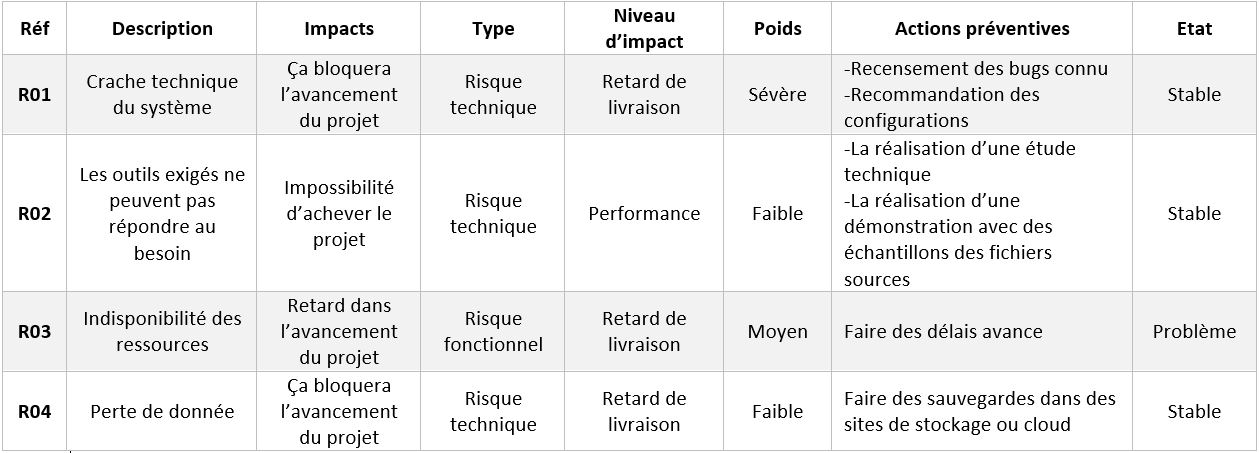
\includegraphics[scale=0.5,keepaspectratio]{Rapport de stage PFE chez DXC/figures/risques.jpg}
    \caption{Registre de Gestion des Risques}
\end{figure}

\section{Déroulement du projet}

\subsection{Methodologie Scrum}

Nous avons opté pour cette méthode car la mise en œuvre de notre projet nécessite une vision globale de la solution à mettre en place, que ce soit au niveau technique, architectural ou fonctionnel. De plus le projet n’est décrit que par des phases clés lors de son développement, les besoins de client se concrétisent à la phase de réalisation, chose qu’on ne peut jamais fixer à l’avance par la modélisation initiale, ajoutant a cela l’extensibilité du système dans le temps, la demande de nouvelle fonctionnalités ..etc. la méthode agile qui permet une vérification fonctionnelle tout en recueillant les nouveau besoins s’est montré indispensable dans ce cas, en plus c’est la méthode demandée par l’entreprise, j’étais dans l’obligation de respecter les consignes de mon employeur et de travailler avec.

\begin{figure}[!h]
    \centering
    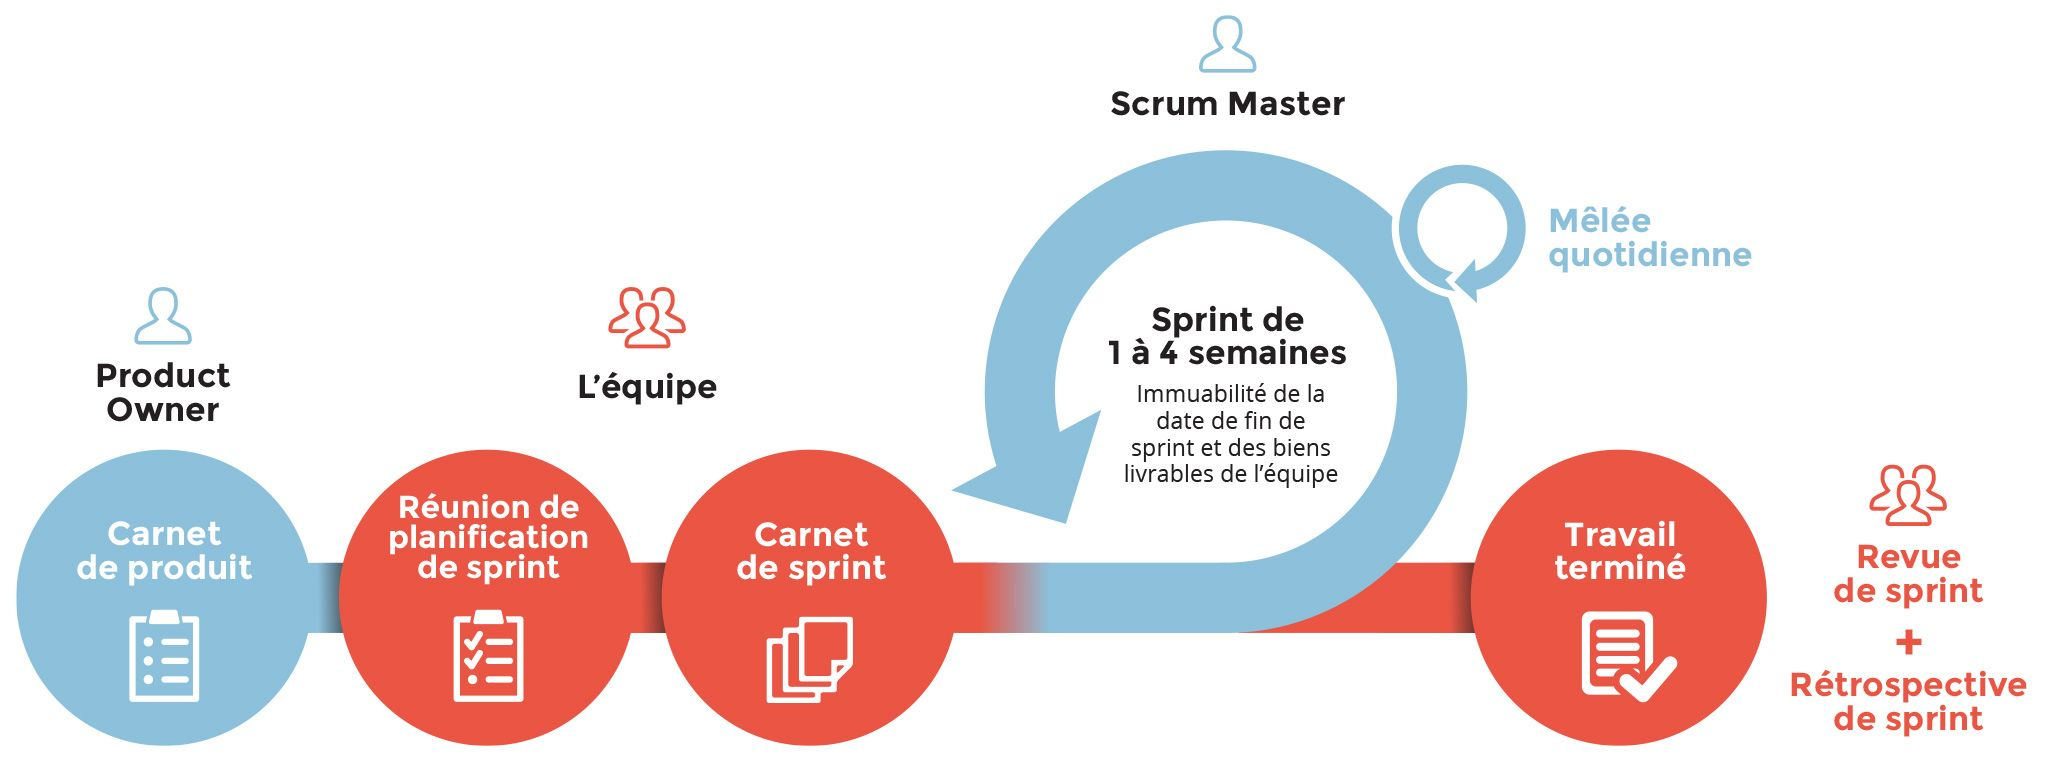
\includegraphics[scale=0.25,keepaspectratio]{Rapport de stage PFE chez DXC/figures/scrum-methode.jpeg}
    \caption{Methodologie Scrum}
\end{figure}

\subsection{Méthodologie de développement}

\begin{itemize}
  \item \textbf{Carnet de produit}: 
        Le Product Owner rédige les User Stories et les place dans le Product Backlog.
        Le Product Owner priorise ensuite ces User Stories et ordonne le Product
        Backlog en conséquence.
    \\
    \item \textbf{Réunion de planification de sprint}: 
        L’équipe Scrum se réunit lors de la réunion de planification de Sprint afin
        d’établir la liste des User Stories qui seront traitées pendant le Sprint. Celles-ci
        constituent le Sprint Backlog et sont ensuite découpées en tâches par l’équipe
        de développement.
    \\    
    \item \textbf{Début de Sprint}: 
        Le Sprint peut alors commencer pour une itération de 2, 3 ou 4 semaines.
    \\    
    \item \textbf{Mêlée quotidienne}: 
        L’équipe se réunit quotidiennement pour réaliser la Mêlée quotidienne
    \\    
    \item \textbf{Fin de sprint}: 
        À l’issue du Sprint, nous possédons un produit potentiellement livrable qui fait l’objet d’une démonstration lors de la revue du Sprint.
    \\    
    \item \textbf{Rétrospective de Sprint}: 
        Le cycle se termine enfin par la rétrospective de Sprint. Et ensuite, il n’y a plus qu’à répéter tout cela…
\end{itemize}

\subsection{Phases du projet}

La partie suivante présente les différentes phases par lesquelles est passé le projet à savoir :
\\

\begin{itemize}
  \item \textbf{Phase initialisation et cadrage: }
        Dont les taches sont la prise de connaissance du contexte et métier de
        l’entreprise cliente et l’environnement du projet.
    \\
    \item \textbf{Etude technique et fonctionnelle}: 
        Qui a pour but d’installer l’environnement du travail, tenir des réunions avec les responsables, rédiger les spécifications fonctionnelles et fixer les choix fonctionnels à travers un document de spécifications des besoins découlant de l’analyse et des besoins du client.
    \\    
    \item \textbf{Réalisation de l’application}: 
        Cette étape constitue l'étape active de la démarche de projet en ce sens où
        elle concrétise la réalisation du projet, c'est pendant cette étape que se réalisent toutes les prévisions définies précédemment et que s'engagent les ressources dimensionnées durant l'étape de conception.
    \\    
    \item \textbf{La mise en production de cette application}: 
        Déploiement de l’application après la réalisation des tests dans l'environement de production où le client peut utiliser l’application.
    \\    

\end{itemize}

\subsection{Equipe du projet}
Le projet sera réalisé par un groupe de deux stagiaires et trois employés qui sont les membres de l'equipe Power Platform comme montré dans la figure suivante:
\\

\begin{figure}[!h]
    \centering
    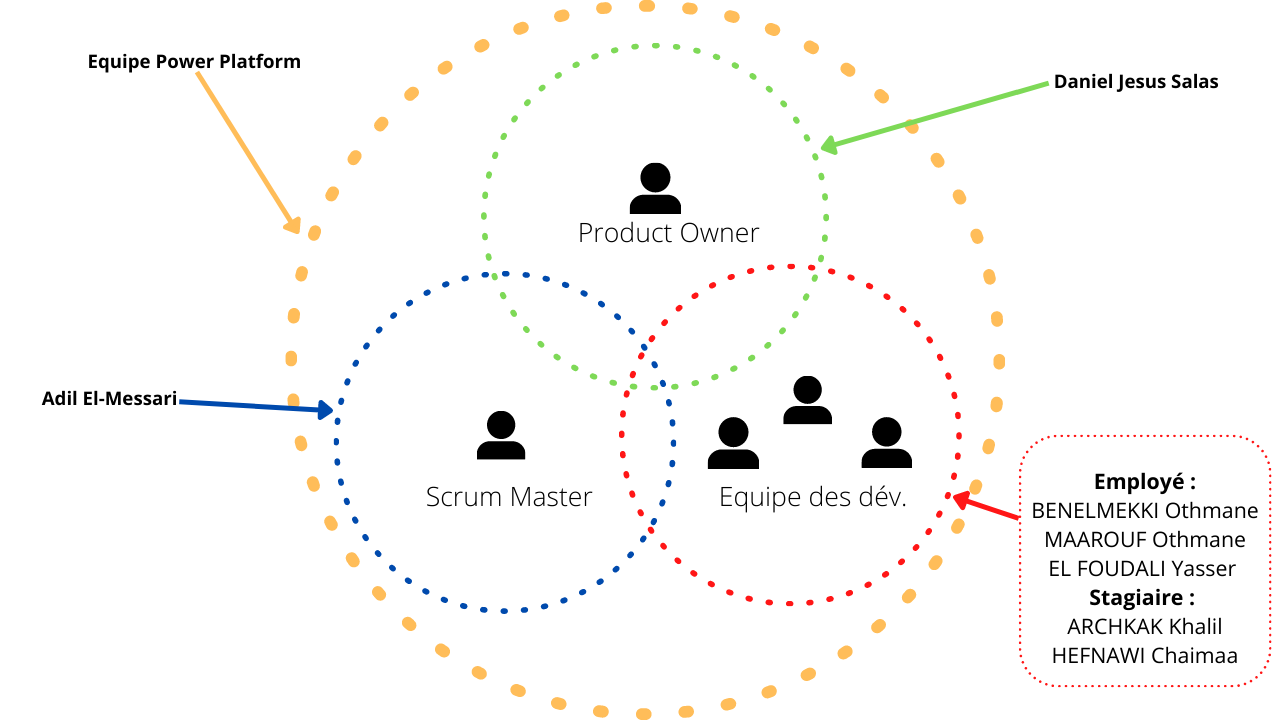
\includegraphics[scale=0.5,keepaspectratio]{Rapport de stage PFE chez DXC/figures/equipe_du_projet.png}
    \caption{Equipe du projet}
\end{figure}

La méthode Scrum définit trois rôles qui sont :
\\

\begin{itemize}
  \item \textbf{Le Product Owner (le propriétaire du produit):}
        c’est une personne qui porte la vision du produit à réaliser, généralement c’est un expert dans le domaine.
    \\
    \item \textbf{Le Scrum Master (le directeur de produit) :}
        c'est la personne qui doit assurer le bon déroulement des différents sprints du release, et qui doit impérativement maitriser Scrum.
    \\    
    \item \textbf{La ScrumTeam (l’équipe de Scrum) :}
        constitué des personnes qui seront
        chargées d’implémenter les différents besoins du client. Bien
        évidemment, cette équipe sera constituée des développeurs, des
        infographistes,etc.
    \\    

\end{itemize}

\subsection{Planification du projet}
Le projet était nouveau pour ma part, Il utilise power platform une technologie non abordée le long de mon parcours scolaire. Du coup, une planification rigoureuse s’est imposée pour prévoir le déroulement du projet.

D'autre part le projet souffre de l'impossibilité de verrouiller les exigences entre les versions et cela est dû à la complexité des processus que le projet tente de résoudre, ce qui entraîne un cycle de changements d'exigences nécessitant un niveau d'agilité plus élevé, la raison pour laquelle Power Platform a été choisi comme choix de technologie.

Le stage a débuté le 1er mars pour une durée de 6 mois. Il en résulte le planning
suivant :

\begin{figure}[!h]
    \centering
    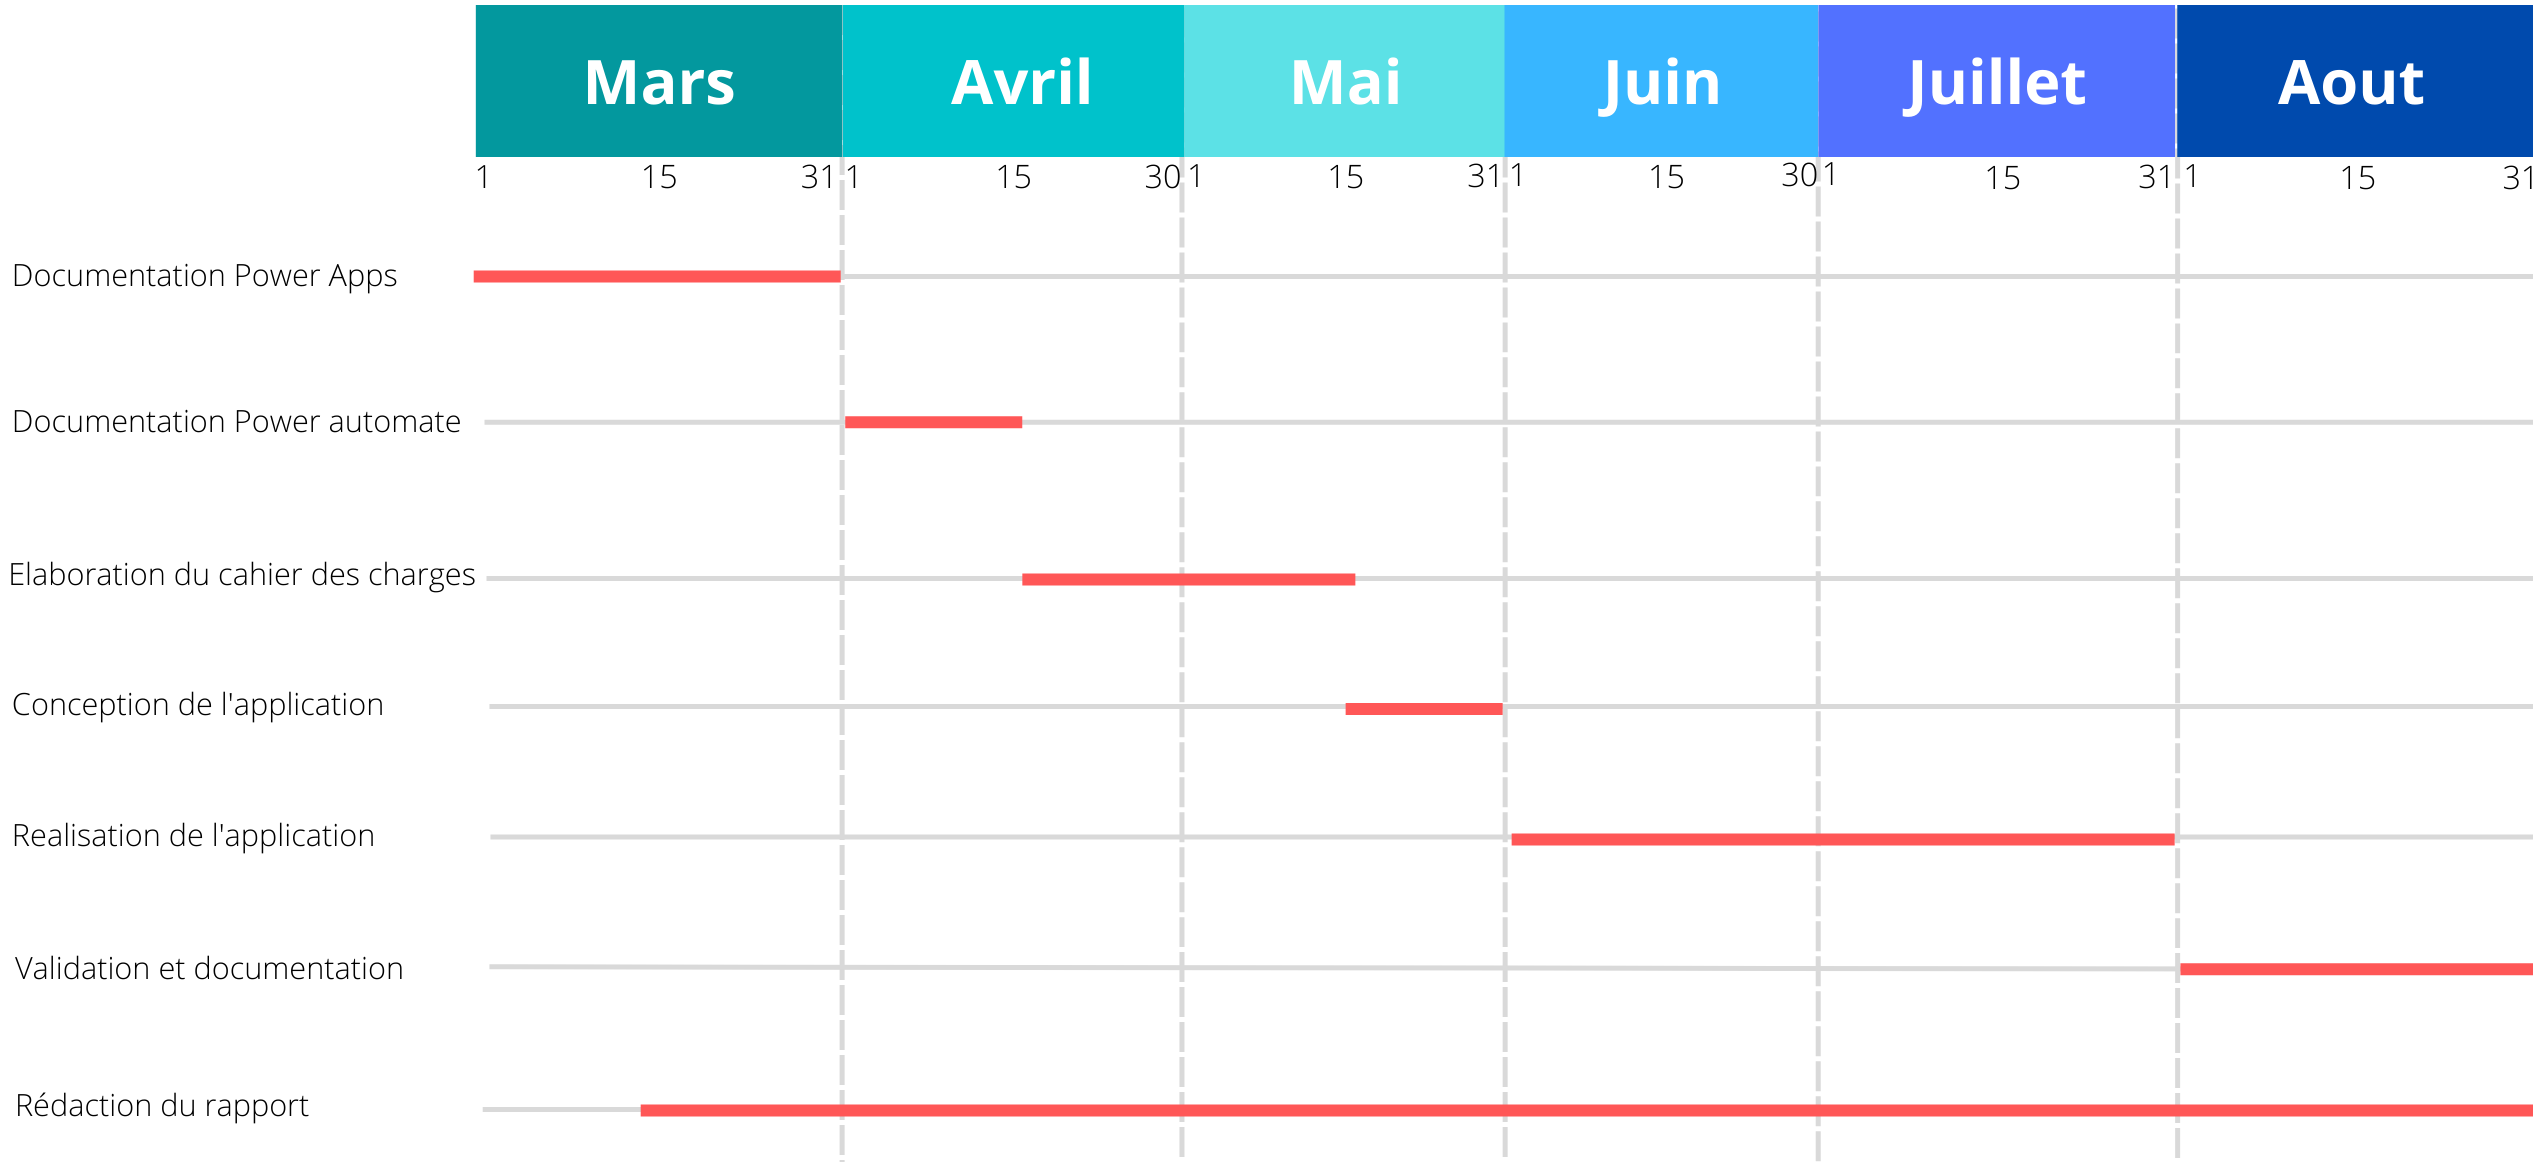
\includegraphics[scale=0.25,keepaspectratio]{Rapport de stage PFE chez DXC/figures/planification_projet_cropped.png}
    \caption{Diagramme de Gantt}
\end{figure}




\\
Le projet est partagé en trois grandes étapes : 
\\
\begin{itemize}
  \item La première est \textbf{une phase de documentation} dont les objectifs était de bien assimiler les différents composant de Microsoft Power Platform.
  \\
  \item \textbf{La phase de l'élaboration du cahier de charge}, vu que le projet avait beaucoup de collaborateur cette dernière a pris du temps pour les mettre en accord sur les différentes fonctionnalités de l'application.
  \\
  \item \textbf{La phase de conception de l'application} qui a permis de construire un systeme qui relie plusieurs entité et outils mais surtout elimine les fichiers Excel du processus.
  \\
  \item \textbf{La phase de réalisation de l'application} où j'ai commencé par d'abord élaborer le frontend pour ensuite passer au backend en utilisant Power Apps et Power Automate.
  \\
  \item Finalement \textbf{la phase de validation de l'application} par les différents membres de l'équipe ainsi que ça documentation.
  \\
\end{itemize}
\\

\subsection{Gestion et suivi du projet}
Pour ce qui est de la gestion et suivi des nouvelle fonctionalité ainsi qu'erreur dans le projet. \textbf{Azure Boards} était l'outil utilisé pour permettre ce suivi.

Cette image represente quelque elements du backlog :

\begin{figure}[!h]
    \centering
    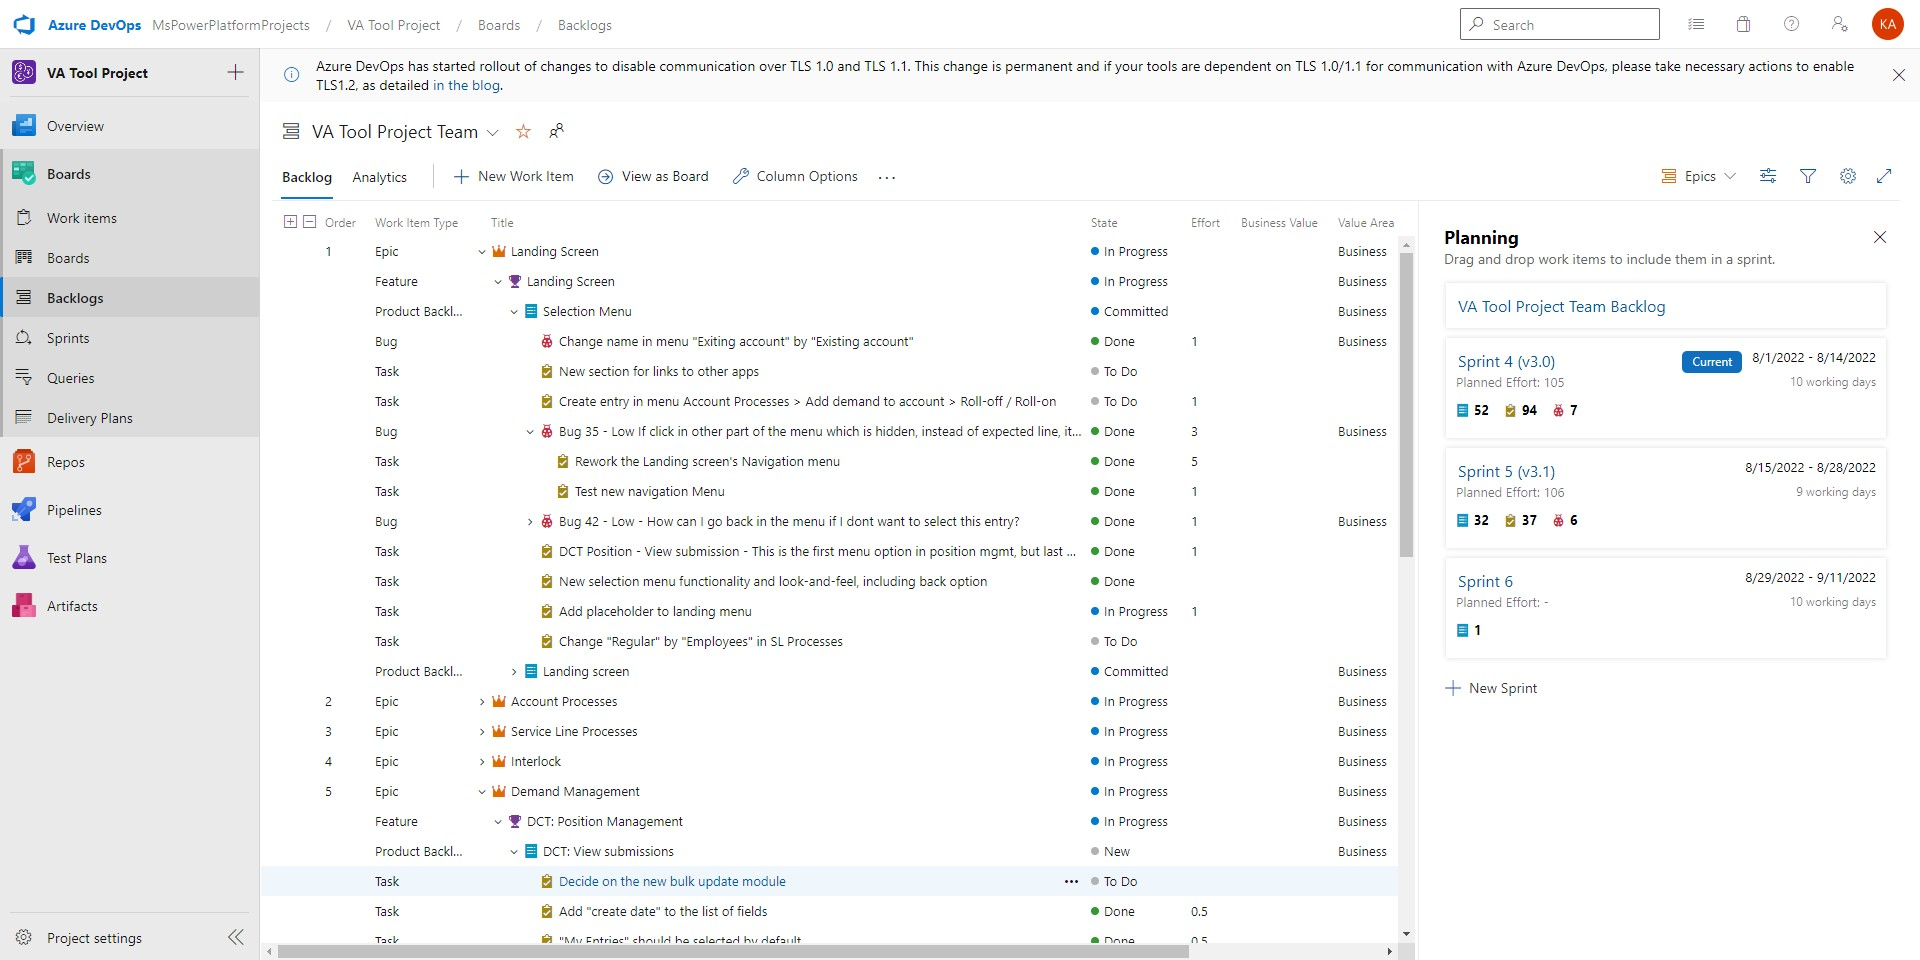
\includegraphics[scale=0.32,keepaspectratio]{Rapport de stage PFE chez DXC/figures/AzureBoards_Backlog.jpg}
    \caption{Azure Boards : Backlog}
\end{figure}

Pour hiérarchiser notre projet nous avons utilisé 4 catégories dans Azure Boards :
\\

\begin{itemize}
  \item \textbf{Epic:} Représentant un module ou un groupe de fonctionnalité.
  \\
  \item \textbf{Feature :} Représentant les différentes fonctionnalités voulu pour le module.
  \\
  \item \textbf{Product backlog Item :} Qui représente les screens qui vont être créer pour ce module.
  \\
  \item \textbf{Tasks:} Ensuite viens les taches qui vont être effectué pour la création de ces derniers.
\end{itemize}

\\\\

A part cela nous avons aussi utilisé deux autres catégories :
\\

\begin{itemize}
  \item \textbf{Bug :} Pour le suivi et l’assignation des nouveau bugs trouvé.
  \\
  \item \textbf{Test Case :} Pour le testing des fonctionnalités de l’applications.
\end{itemize}

\vspace{\baselineskip}
Après avoir définit les différents items dans le backlog vient l'étape du verrouillage des différents items qui seront inclus dans le sprint de développement, le Product Owner ainsi que le Scrum Master discute des priorités des différentes taches et les ajoute en se basant sur cette dernière au sprint de développement.
Ensuite vient l'étape d'estimation des efforts nécessaire pour chaque tache pour ne pas dépacer la capacité de l'équipe de développement et ne pas pouvoir terminer toutes les taches du sprint, L'estimation se fait avec des sessions de planning poker.Donc après le sprint planning la phase de réalisation et d’implémentation démarre en assignant chaque tâche à une personne.


\begin{figure}[H]
    \centering
    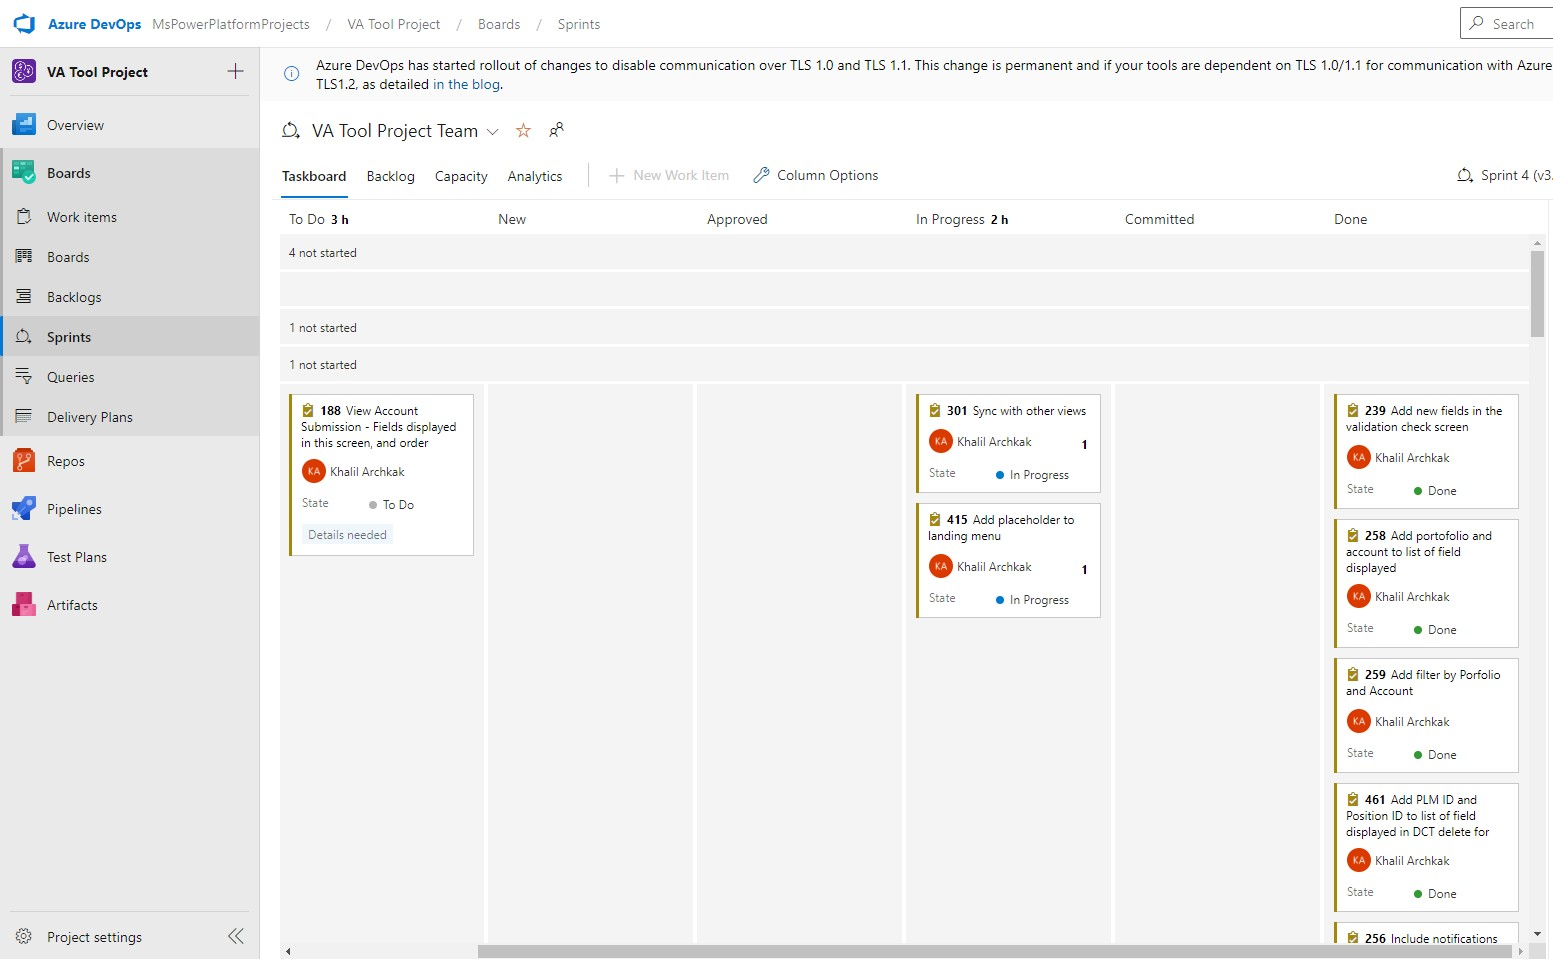
\includegraphics[scale=0.34,keepaspectratio]{Rapport de stage PFE chez DXC/figures/Sprint_TaskBoard.jpg}
    \caption{Azure Boards : Sprint Task Board}
\end{figure}

Tous les matins à 9H on fait une réunion qui regroupe l'équipe de développement ainsi que le Product Owner et le Scrum Master sur Microsoft Teams dans laquelle on discute de ce qu’on a fait hier et ce qu’on va faire aujourd’hui et les points de blocage, ces derniers sont listés dans une carte Trello comme le montre la figure suivante :

\begin{figure}[H]
    \centering
    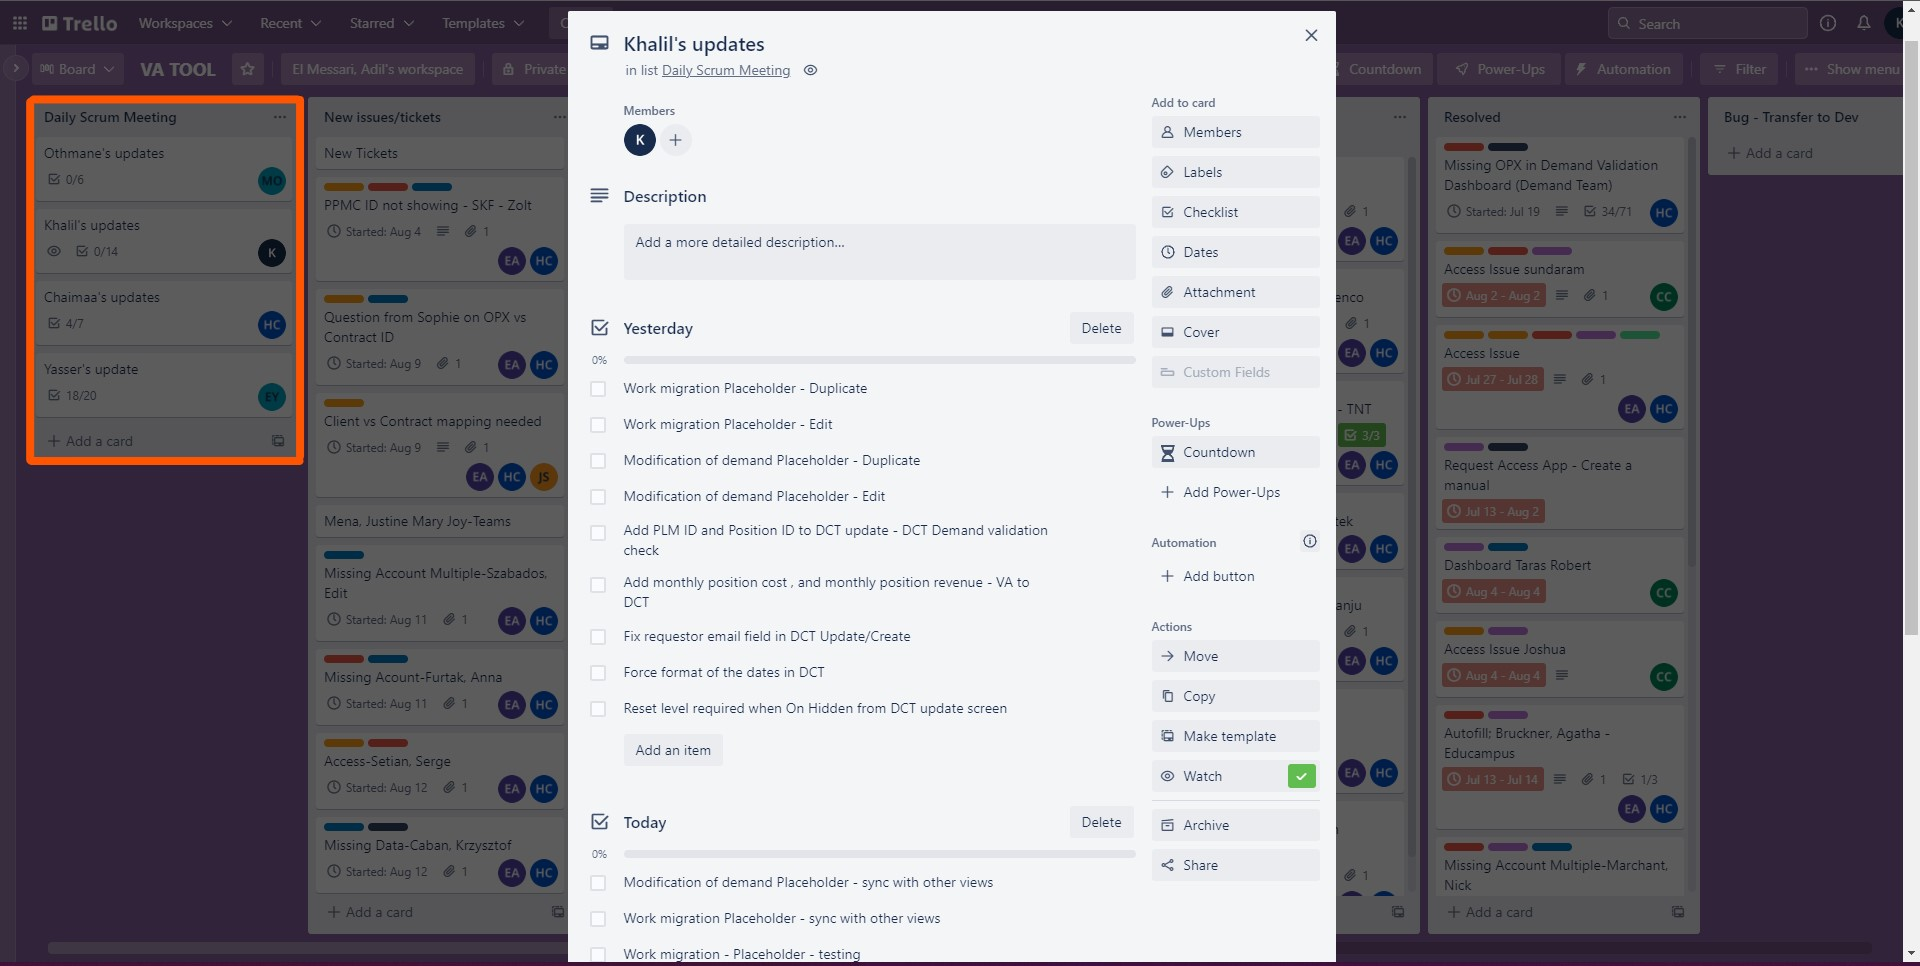
\includegraphics[scale=0.28,keepaspectratio]{Rapport de stage PFE chez DXC/figures/Trello_Daily.jpg}
    \caption{Trello : Daily meetings}
\end{figure}




\section{Conclusion}

Dans ce chapitre j’ai présenté l’étude générale du projet et le choix de la méthodologie ainsi
que le déroulement du projet,son but, les differents livrable, la planification du projet, et finalement la gestion et suivi de ce dernier. Le chapitre suivant se concentrera sur l’étude des besoins du projet.
